\Chapter{Folyamat példák}

\Section{Áttekintés}

Ez a fejezet bemutatja néhány példa segítségével, hogy hogyan és milyen folyamatokat lehet a program elkészülte után annak használatával modellezni. A példák mellé leírás is társul, hogy érthető legyen a modellezett folyamat.

\Section{Első példa}

Először nézzünk egy, már létező példát arra, hogy hogyan is néz ki egy olyan folyamatábra, amely egy üzleti folyamatot modellez. Ehhez tekintsük az alábbi \textit{BPMN} (Business Process Model and Notation) diagramot (\ref{fig:bpmn} ábra).

\begin{figure}[h]
\centering
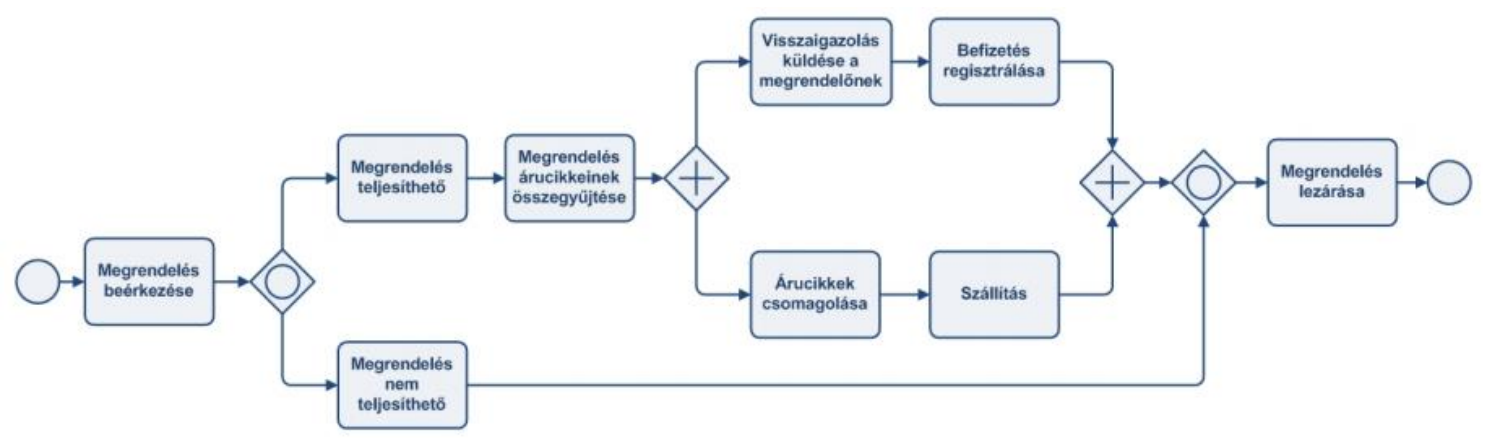
\includegraphics[scale=0.38]{images/BPMN.png}
\caption{BPMN diagram (forrás: \cite{bpmn})}
\label{fig:bpmn}
\end{figure}

Az ábra egy kiváló példa teljes folyamatábrára: Van egy-egy kezdő- és végállapota, minden csomópontba el lehet jutni, és bármelyik csomópontból a végállapotba mehetünk a vonalak és a csomópontok mentén.

A folyamatábrán egy megrendelési folyamatot láthatunk. Első lépésben az adott vállalathoz beérkezik az általuk megrendelt áru. Itt máris útelágazáshoz érkezünk: ha a megrendelés nem teljesíthető valamilyen oknál fogva (például aktuálisan nincs rá kapacitása a cégnek vagy nincs jelen az a személy, aki a megrendeléseket kezeli), akkor máris lezárásra kerül, és végállapotba jutunk a folyamatábrán. Ha viszont minden feltétel adott a megrendeléshez, akkor az teljesíthető. Ekkor összegyűjtik a megrendelés árucikkeit. Ezt követően egy újabb átjáró (vagy elágazás) következik. Láthatjuk, hogy az eddigi két rombusz elem más-más jelölést tartalmaz. Az előbbi egy eldöntendő (igaz vagy hamis) csomópont volt, utóbbi után pedig párhuzamos feladat végrehajtás következik. Egyfelől az összegyűjtött árucikkeket becsomagolják, majd ezt követően elszállítják a megrendelés helyére, ezzel egyidejűleg pedig értesítik a megrendelőt egy visszaigazolással, és regisztrálják a befizetést. Két újabb rombusz alakzat zárja az azonos jellel megjelölt korábbi útválasztó csomópontokat, és végül lezárásra kerül a megrendelés. Az egész folyamat pedig egy kezdő- és egy végállapot közé van fogva.

A fenti ábra után tekintsük meg a \ref{fig:bpmn1} ábrán, hogy pontosan ugyanez a folyamat hogyan modellezhető a szakdolgozat programjának segítségével.

\begin{figure}[h]
\centering
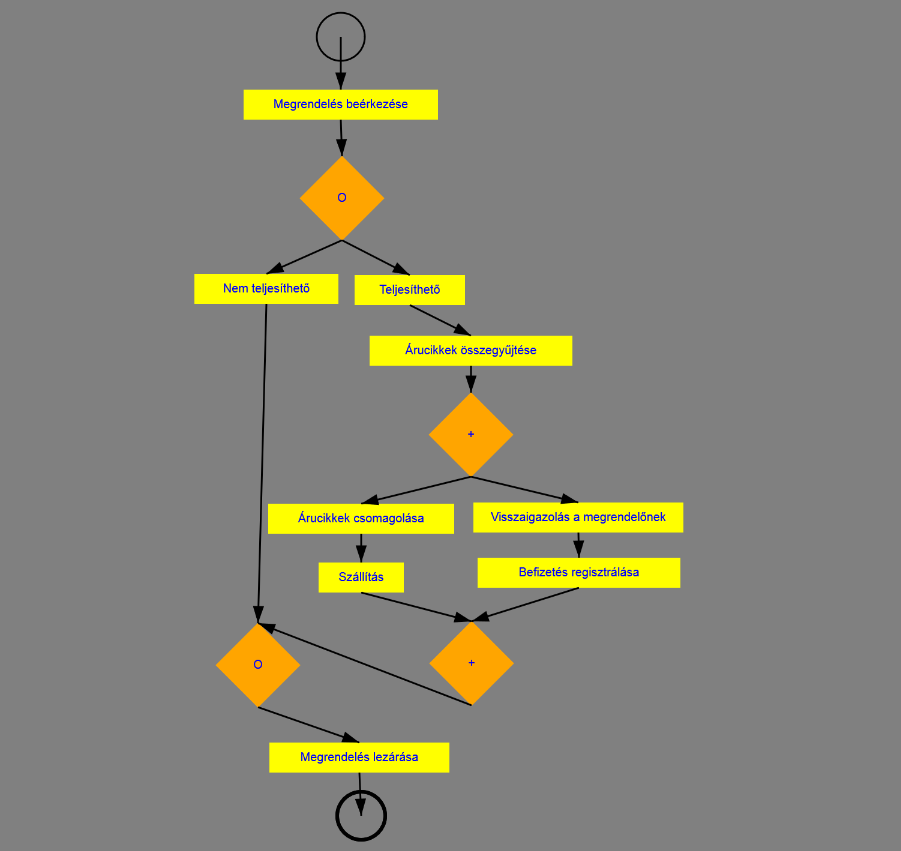
\includegraphics[scale=0.6]{images/pelda1.png}
\caption{BPMN diagram a saját programmal készítve}
\label{fig:bpmn1}
\end{figure}

Némi eltérés felfedezhető a két ábra között. A szakdolgozat alkalmazás színes csomópontokat használ, ami látványosabbá teszi a modellezést, azonban azok összekötésére kisebb hangsúlyt fektet. Előbbi ábrán a csomópontok szövegei több sorba való tagolással vannak megvalósítva, így minden tevékenységet jelölő csomópont azonos méretű. Hosszabb szövegek esetén viszont már nem lesz meg ez az egység. A szakdolgozat programjában ellenben minden csomópont pontosan azonos méretűre hozható a benne lévő szöveg hosszától függetlenül.

\Section{Második példa}

Második példaként hozzunk létre egy létező diagram mintától függetlenül egy folyamatábrát. Tekintsünk egy szerződéskötési folyamatot, melyhez a(z) \cite{xflowutolso} forrásban leírtakat veszem alapul, amely forrás a dolgozat 2. fejezetéhez hasonlóan a(z) \cite{xflower} hivatkozásban található egyik blogbejegyzés.

A folyamat előfeltétele, hogy már egy korábbi (ajánlattevési) folyamatot az ügyfél, akivel a szerződéskötés esedékes, elfogadott. Ezt követően kerül sor a pontos megegyezés (vagyis a szerződés) írásos formában való rögzítésére. Ennek egy egyszerű folyamatát írja le a forrásban említett blogbejegyzés az alábbi lépésekkel:

\begin{enumerate}
\item Első lépésben vázlatot kell készíteni a megegyezetett feltételek mellett.
\item Ezt követi a vázlat egyeztetése egy ügyvéddel, vagy egy hozzá értő jogi személlyel.
\item Ha jogilag rendben van minden, akkor a megfogalmazott szöveg kiküldése az ügyfél számára a következő lépés.
\item Az ügyfélnek lehetősége van módosításokat kérvényezni, ebben az esetben a feladat ezek felülvizsgálata, a módosítások egyeztetése, visszaküldése az ügyfélnek.
\item A módosítások után célszerű ismét leellenőrizni, hogy jogilag a helyén van-e a szerződéstervezet.
\item Ha ez is megtörtént, már csak jóvá kell hagynia a két félnek a szerződést, azt aláírásukkal hitelesíteni.
\item Végül iktatásra kerül a szerződés, valamint eltárolásra.
\end{enumerate}
A fenti folyamat ábrázolására többféle lehetőségünk is van. Nézzünk rá egy példát (lásd: \ref{fig:bpmn2} ábra).

\begin{figure}[h]
\centering
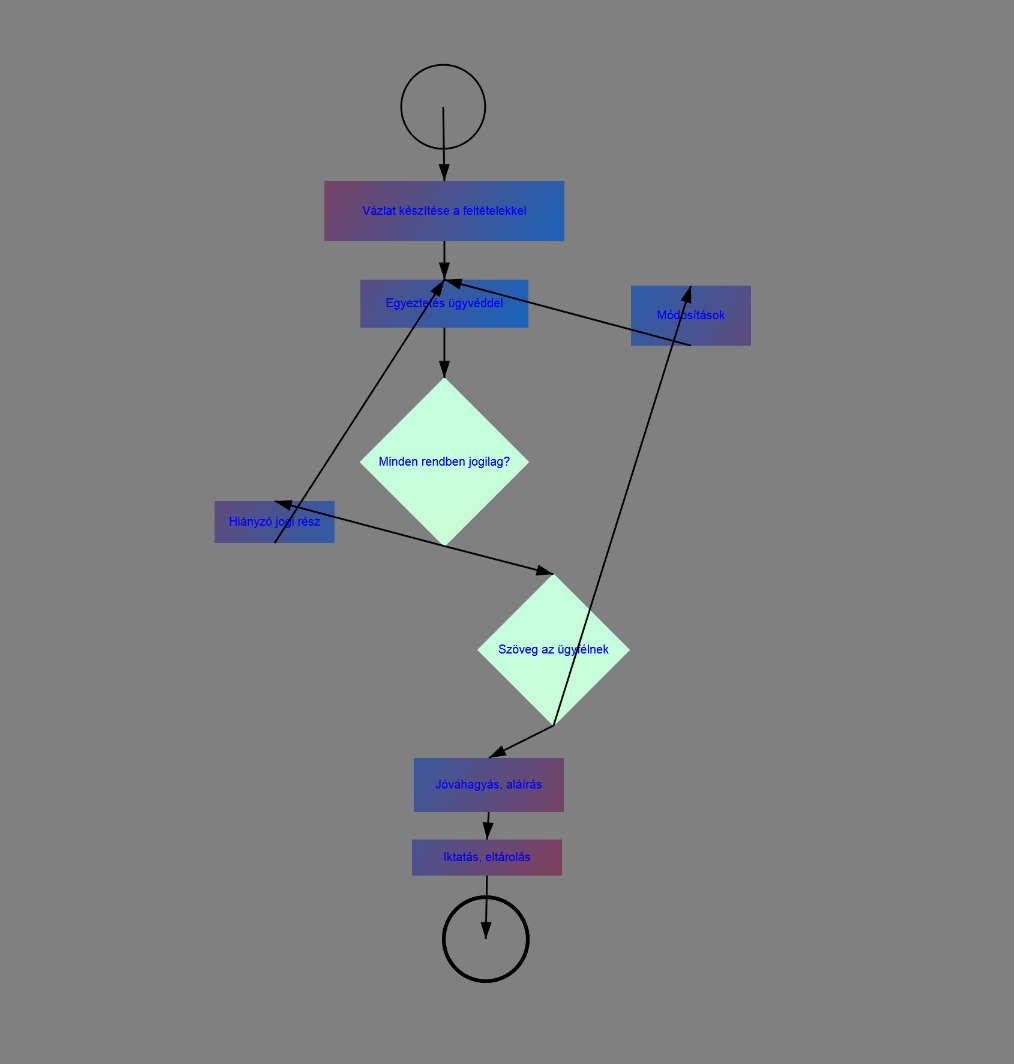
\includegraphics[scale=0.5]{images/pelda2.png}
\caption{Szerződéskötési folyamat modellezése}
\label{fig:bpmn2}
\end{figure}

Először átállítottam a témát, hogy ne csak az alapértelmezett legyen használva, hanem színátmenetes csomópontok is legyenek. Ezután, hogy ne csak tevékenység (téglalap alak) legyen benne, létrehoztam két átjárót is (rombusz alak), ugyanis ha jogi probléma merül fel (például hiányzik a megfogalmazásból valami), akkor ismételten szükség van az ügyvéddel való egyeztetésre, illetve az ügyfélnek küldött szövegen is vagy módosít az ügyfél, vagy következhet a jóváhagyás. Továbbá kihasználtam, hogy a csomópontokat át is lehet méretezni, ezáltal különböző nagyságokat állítottam be az egyes elemeknek.

A fent említett két folyamat példán keresztül még számtalan létezik, és természetesen a felhasználó, aki használni fogja a programot, magától is találhat ki vagy módosíthat kedvére már létező üzleti folyamat modelleket.